% Appendix 
\chapter{NMR Spectra} % Main appendix title

\label{NMR} % Change X to a consecutive letter; for referencing this appendix elsewhere, use \ref{AppendixA}

\begin{figure}[ht!]
\centering
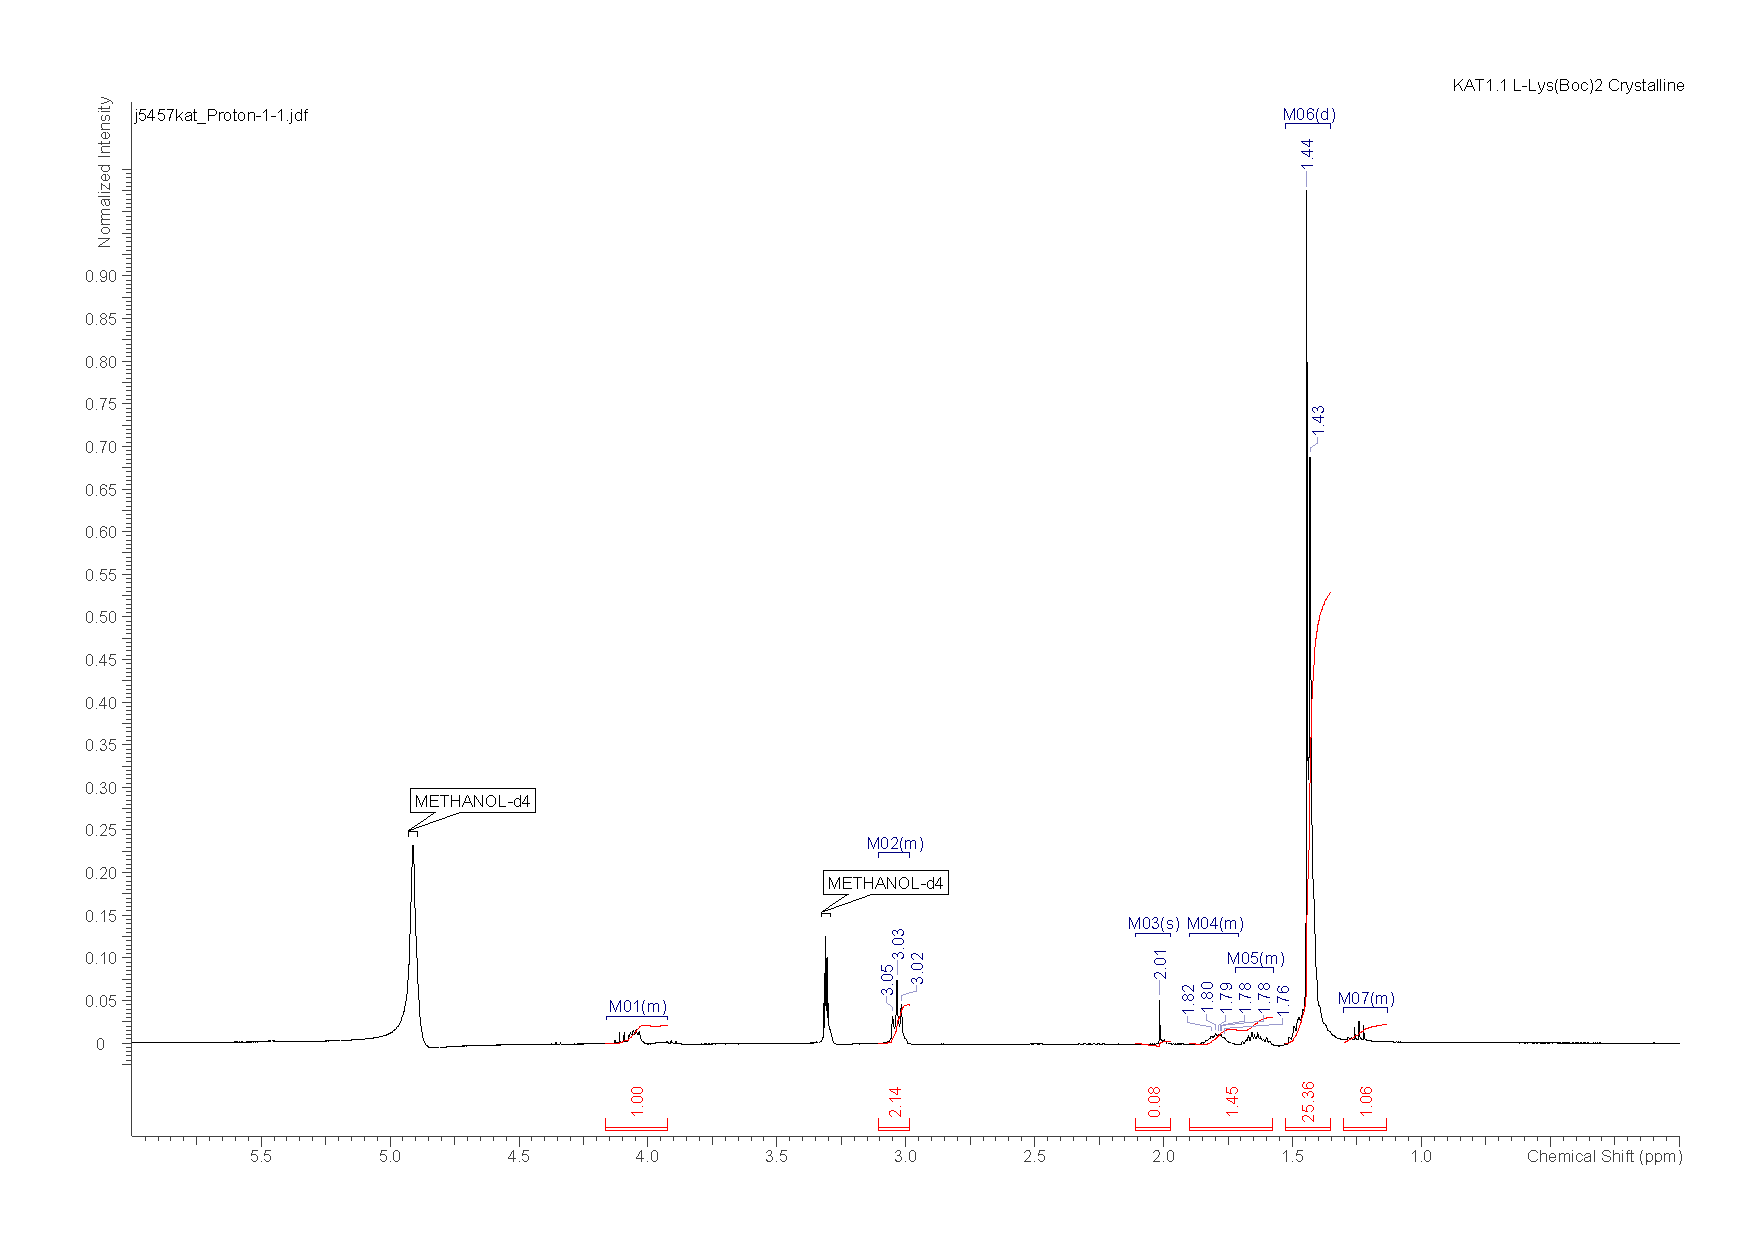
\includegraphics[scale=0.47]{NMR/KAT1_1.pdf}
\caption{\textsuperscript{1}H NMR L-Lys(Boc)\textsubscript{2}}
\label{KAT1.1_NMR2}
\end{figure}

\begin{figure}[ht!]
\centering
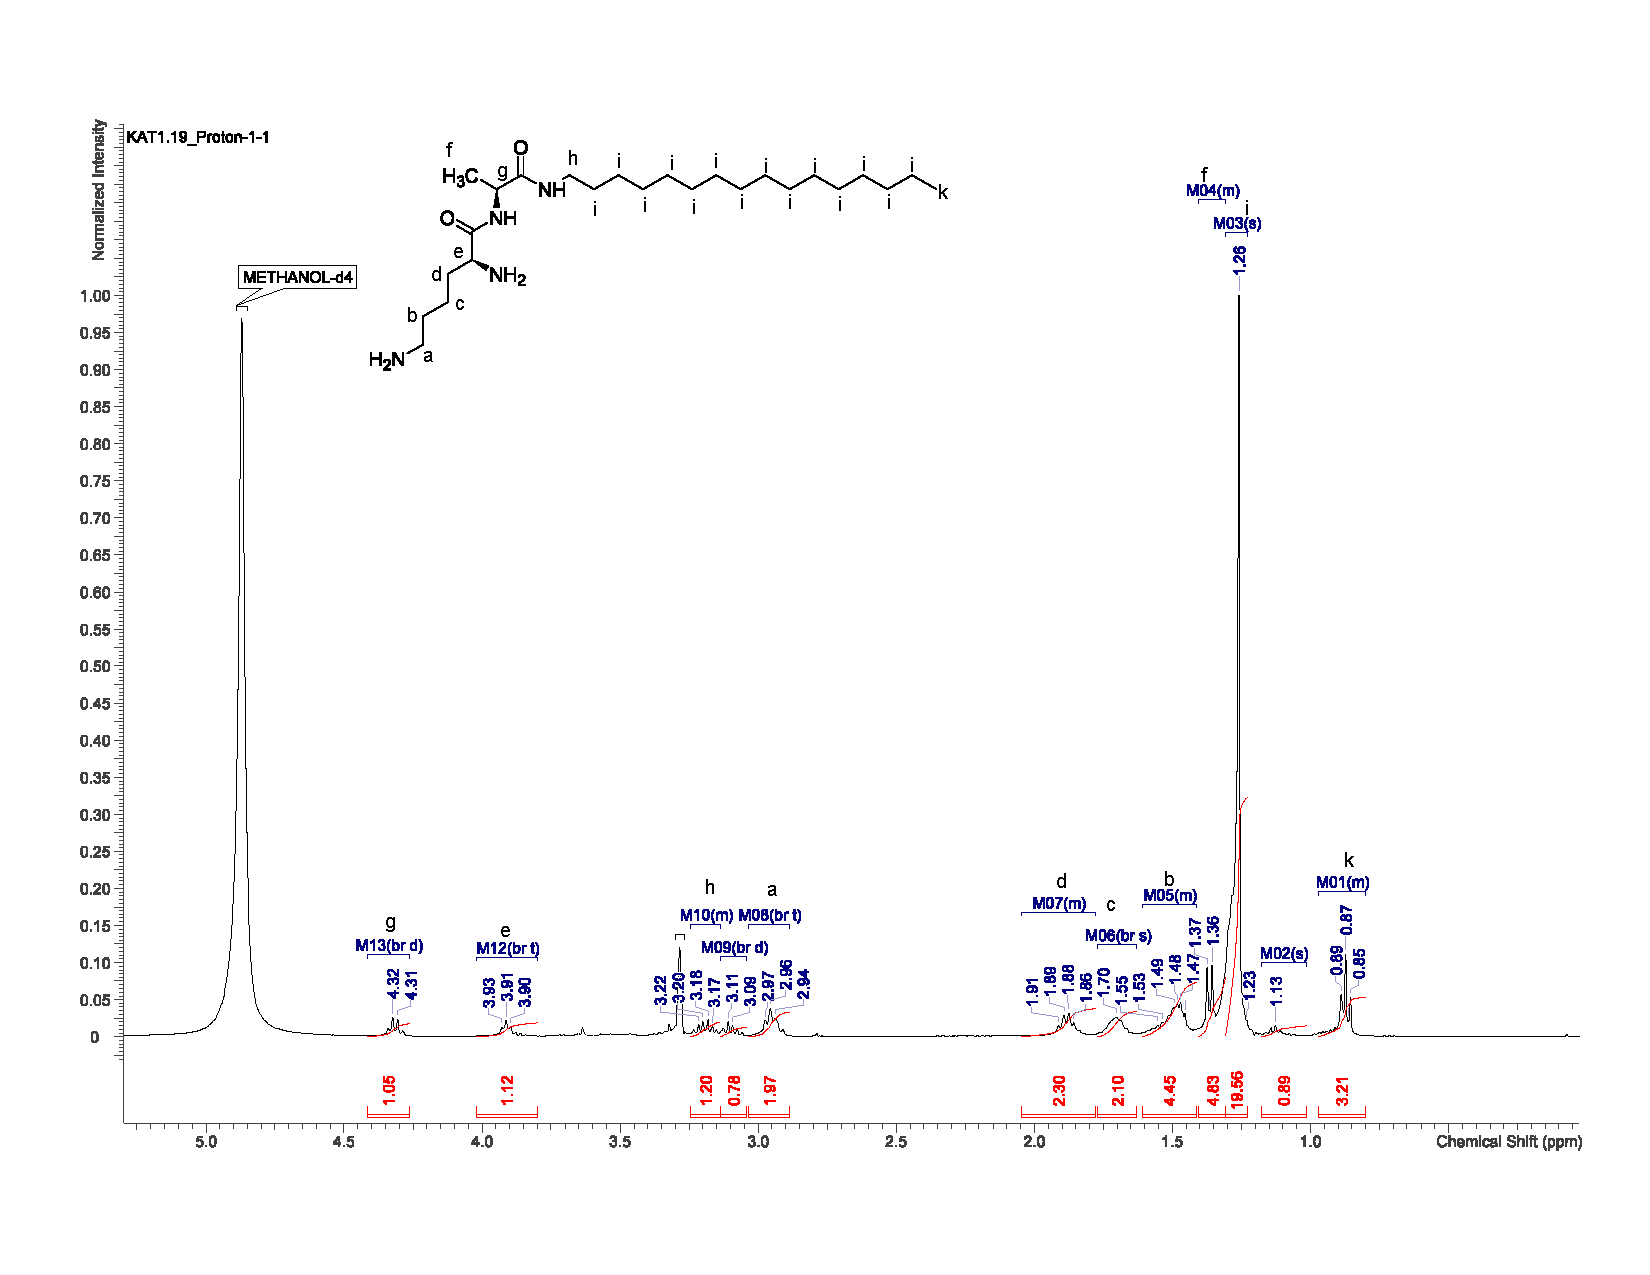
\includegraphics[scale=0.47]{NMR/KAT1_19.pdf}
\caption{\textsuperscript{1}H NMR C16-L-Ala-L-Lys}
\label{KAT1.19_NMR2}
\end{figure}

\begin{figure}[ht!]
\centering
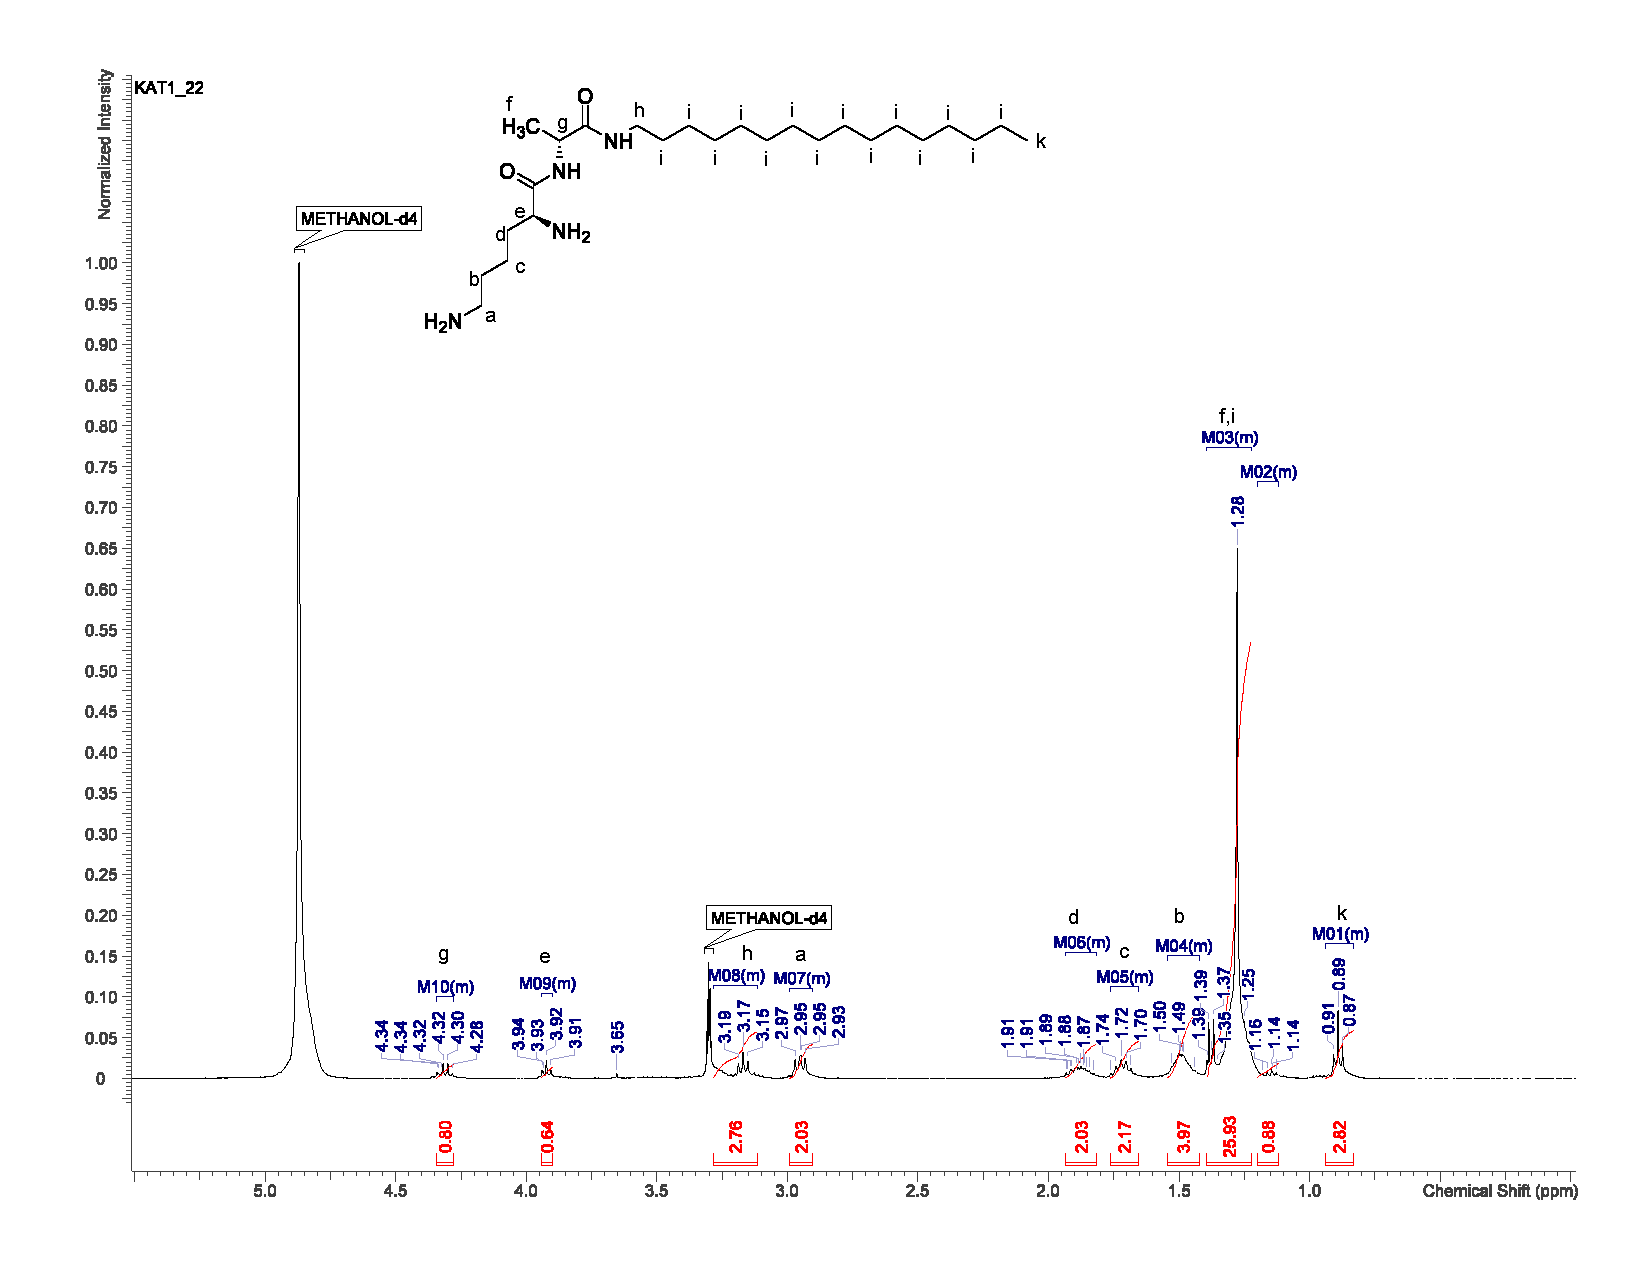
\includegraphics[scale=0.47]{NMR/KAT1_22.pdf}
\caption{\textsuperscript{1}H NMR C16-D-Ala-L-Lys}
\label{KAT1.22_NMR2}
\end{figure}

\begin{figure}[ht!]
\centering
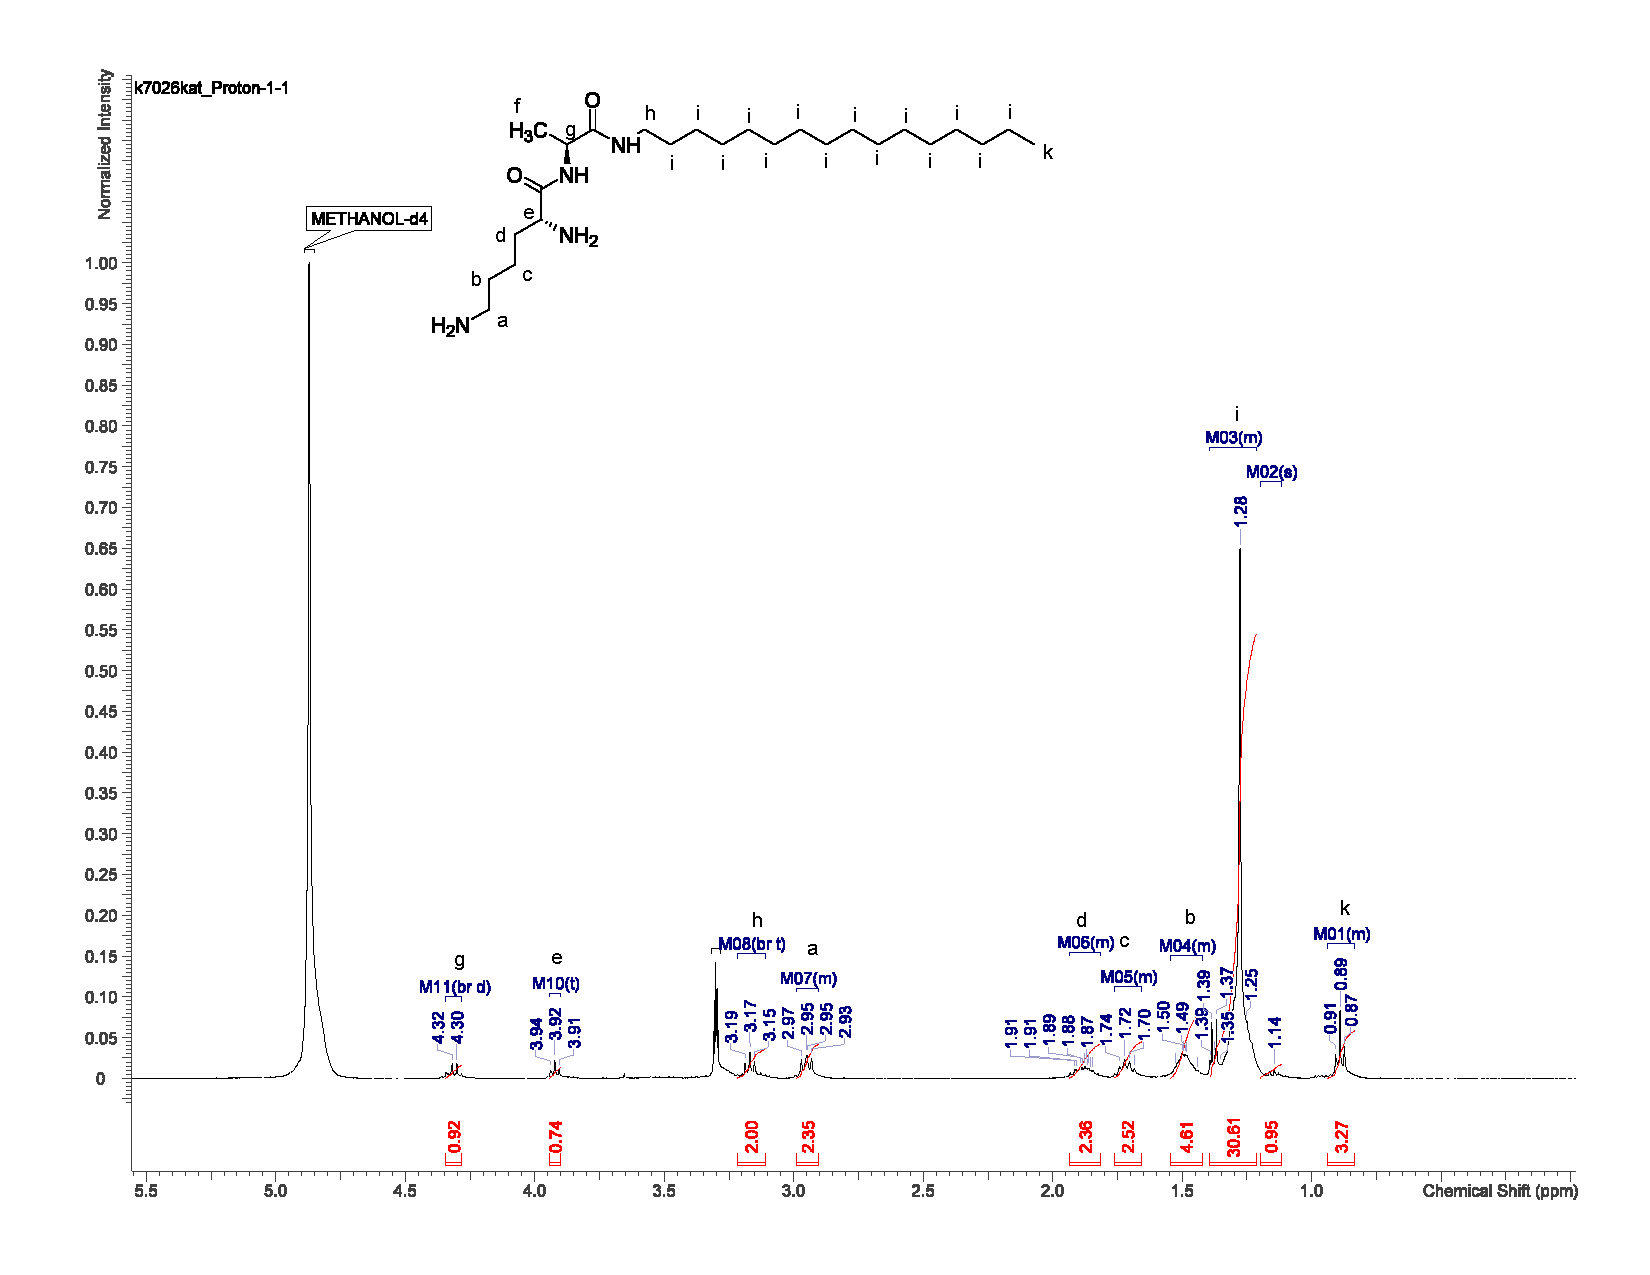
\includegraphics[scale=0.47]{NMR/KAT1_30.pdf}
\caption{\textsuperscript{1}H NMR C16-L-Ala-D-Lys}
\label{KAT1.30_NMR2}
\end{figure}

\begin{figure}[ht!]
\centering
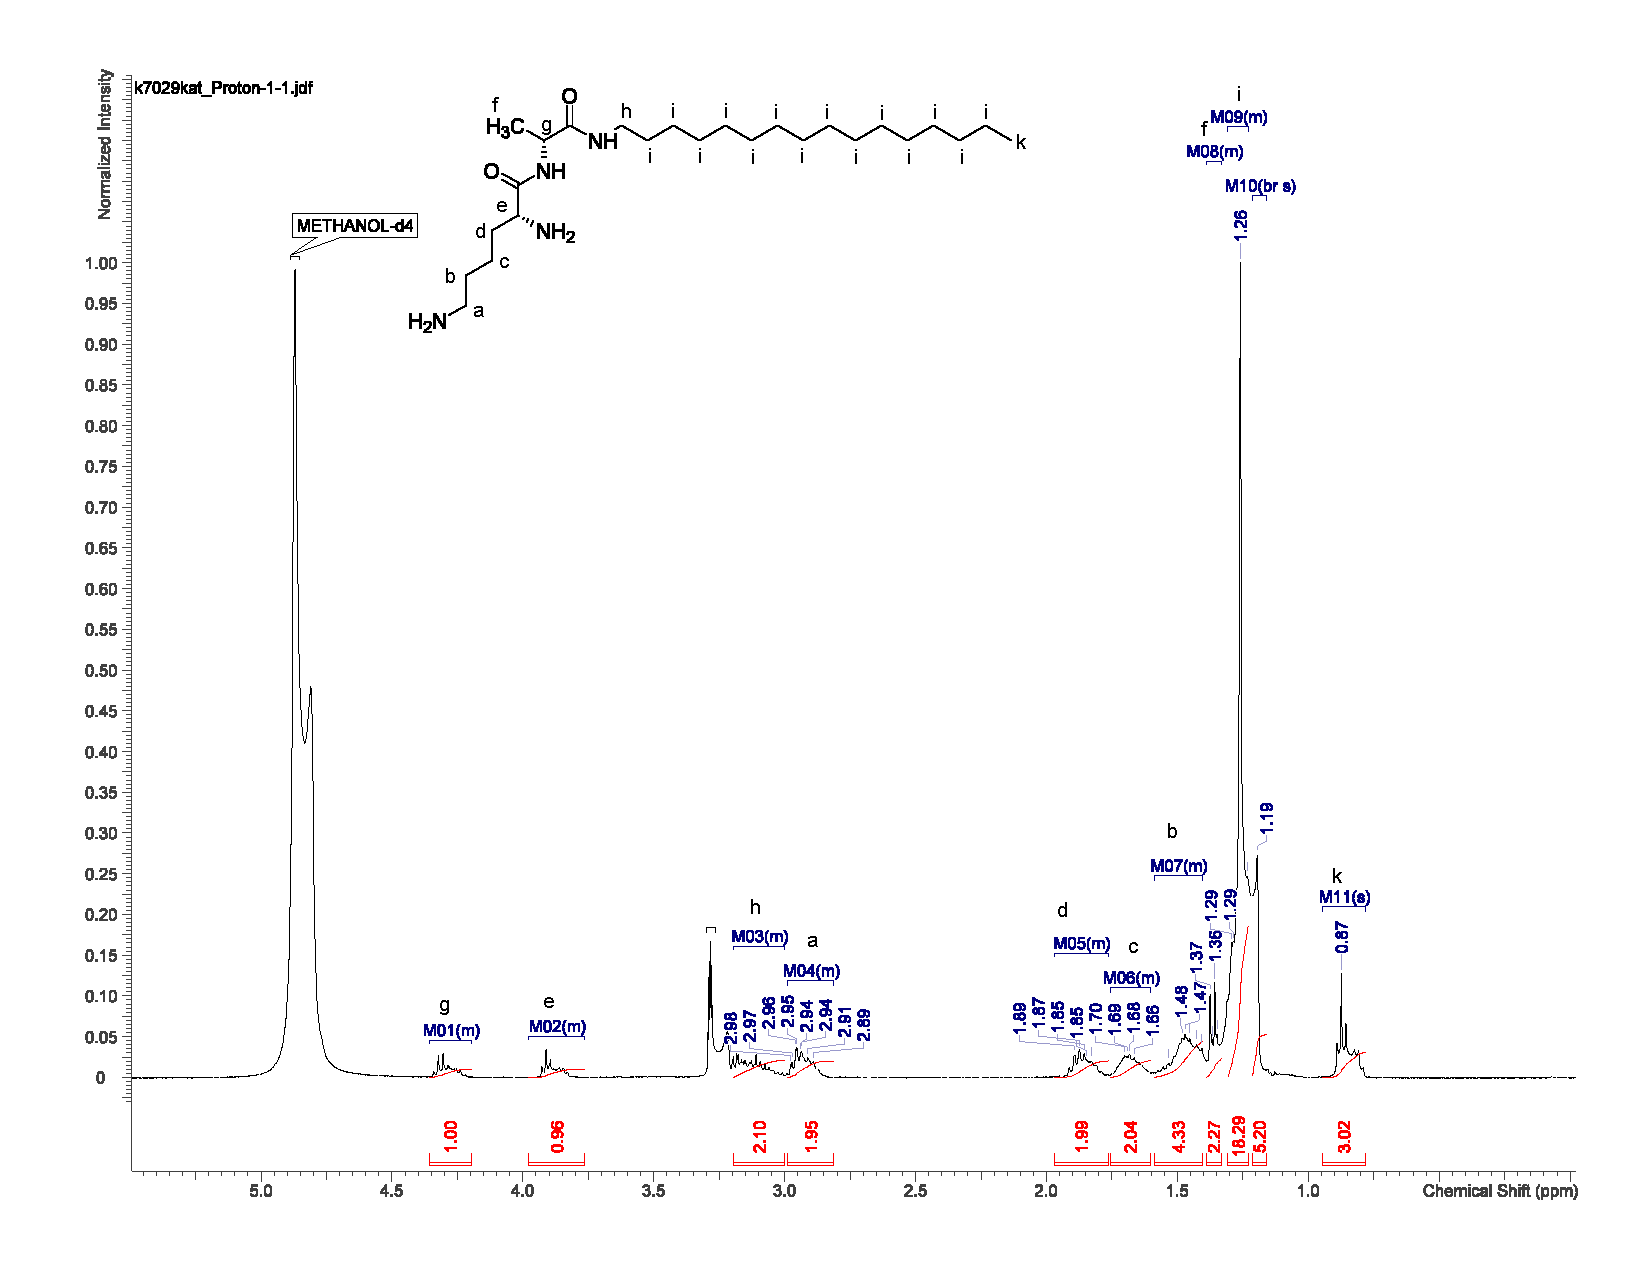
\includegraphics[scale=0.47]{NMR/KAT1_35.pdf}
\caption{\textsuperscript{1}H NMR C16-D-Ala-D-Lys}
\label{KAT1.35_NMR2}
\end{figure}

\begin{figure}[ht!]
\centering
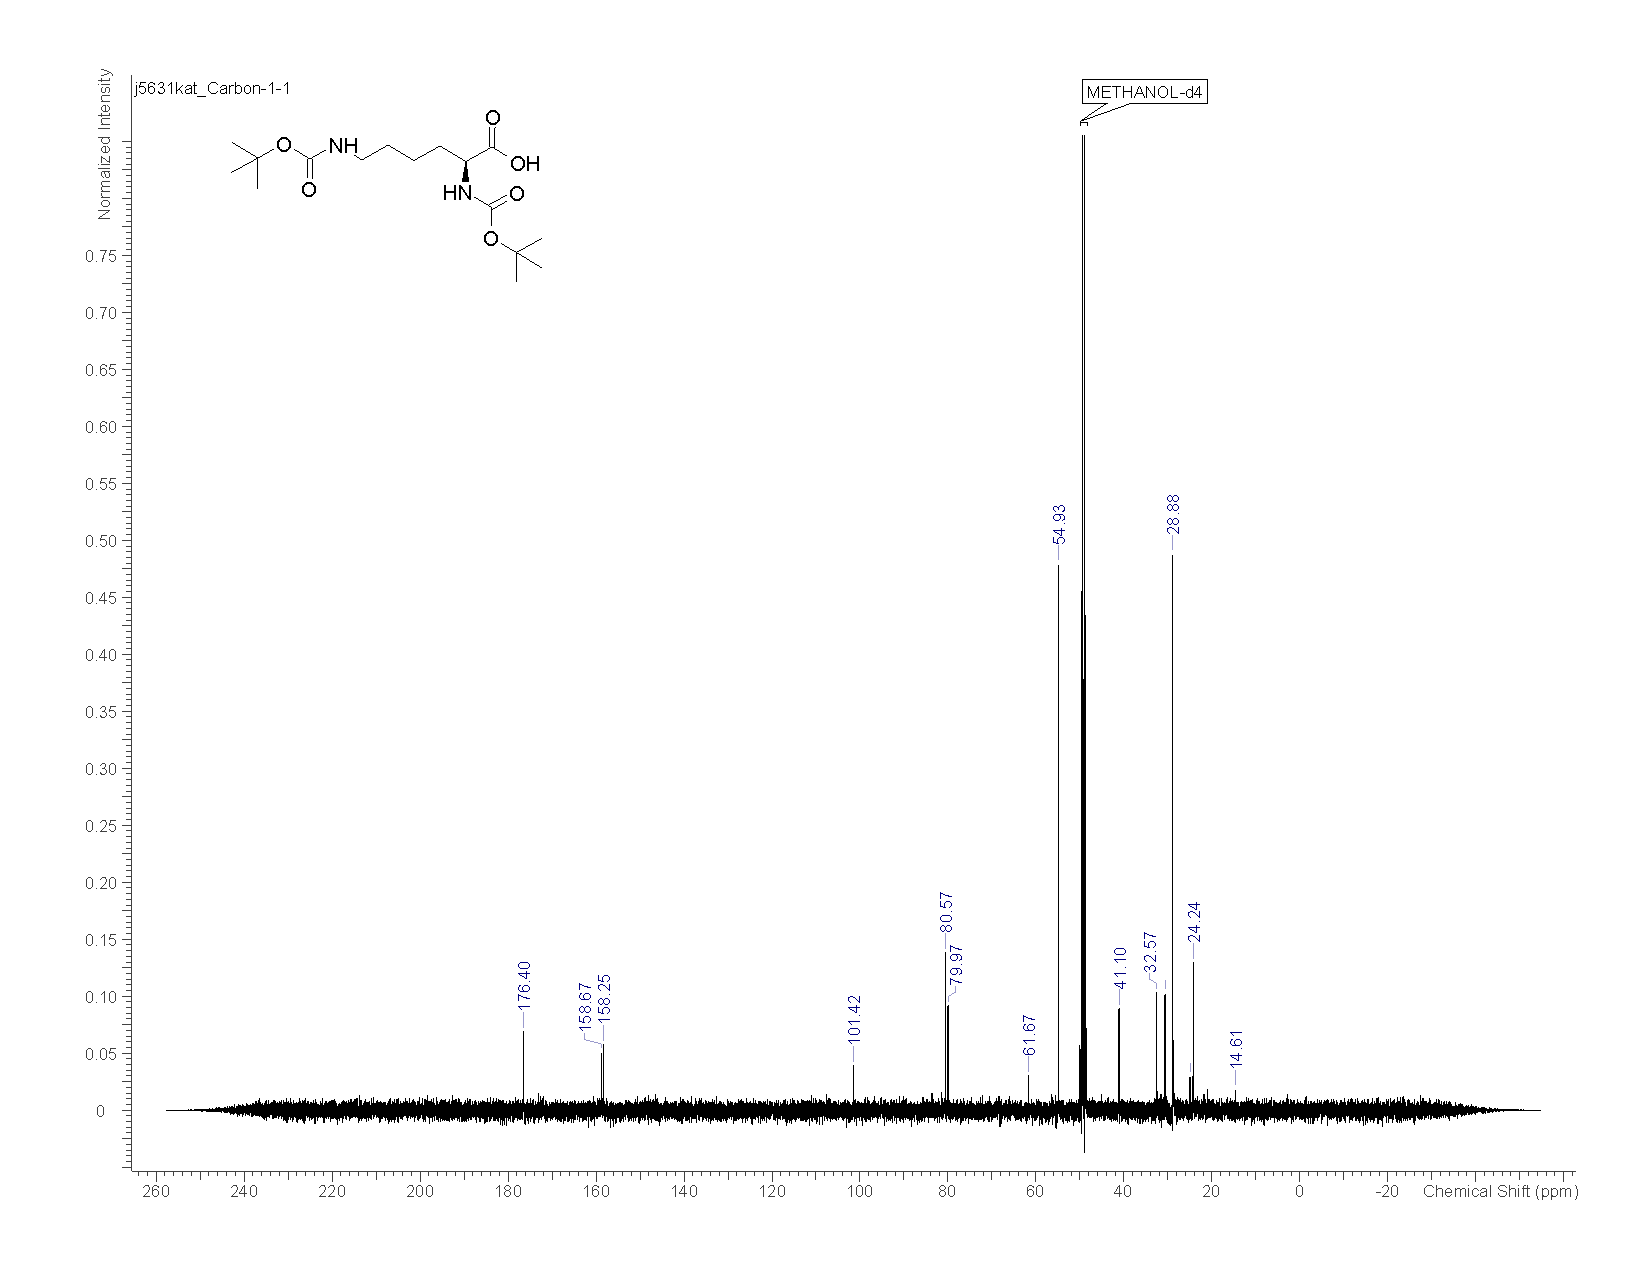
\includegraphics[scale=0.47]{13CNMR/KAT1_1_13C.pdf}
\caption{\textsuperscript{13}C NMR L-Lys(Boc)\textsubscript{2}}
\label{KAT1.1_13C}
\end{figure}

\begin{figure}[ht!]
\centering
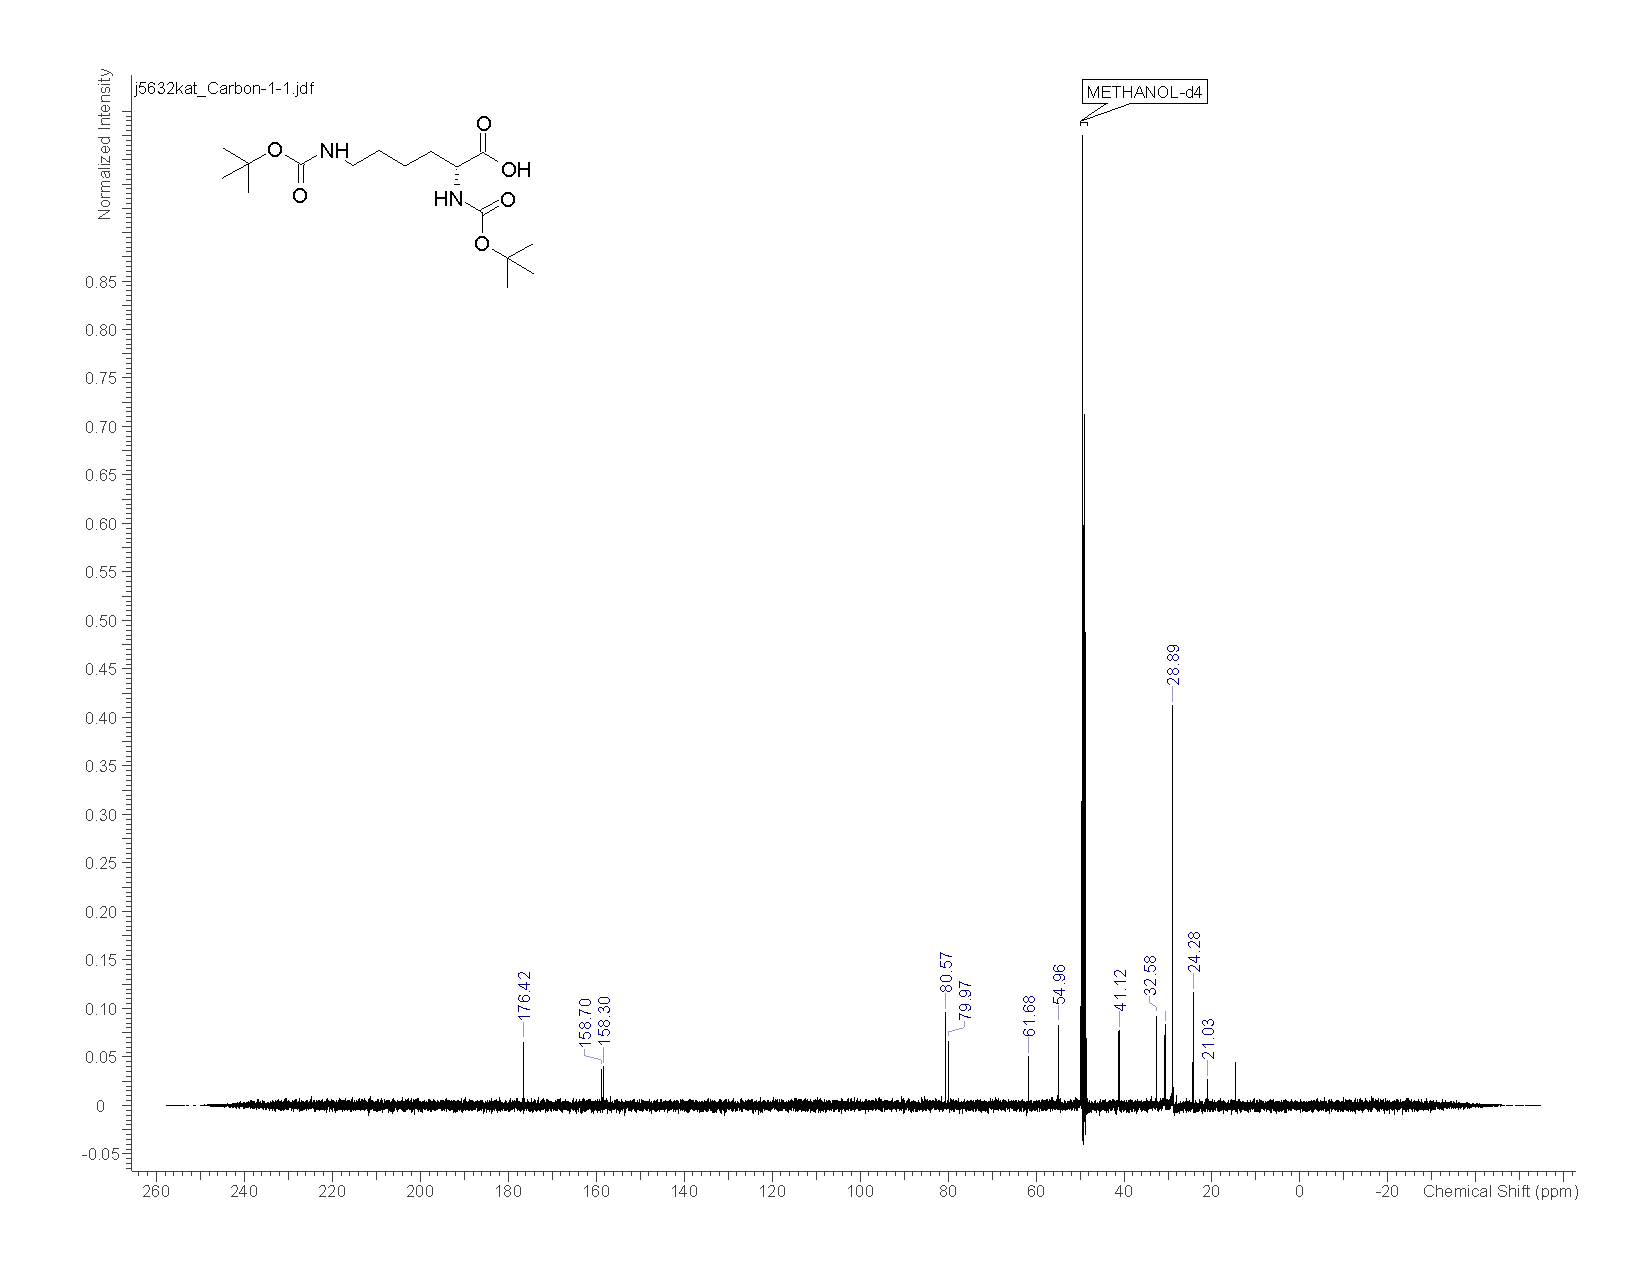
\includegraphics[scale=0.47]{13CNMR/KAT1_5_13C.pdf}
\caption{\textsuperscript{13}C NMR D-Lys(Boc)\textsubscript{2}}
\label{KAT1.5_13C}
\end{figure}

\begin{figure}[ht!]
\centering
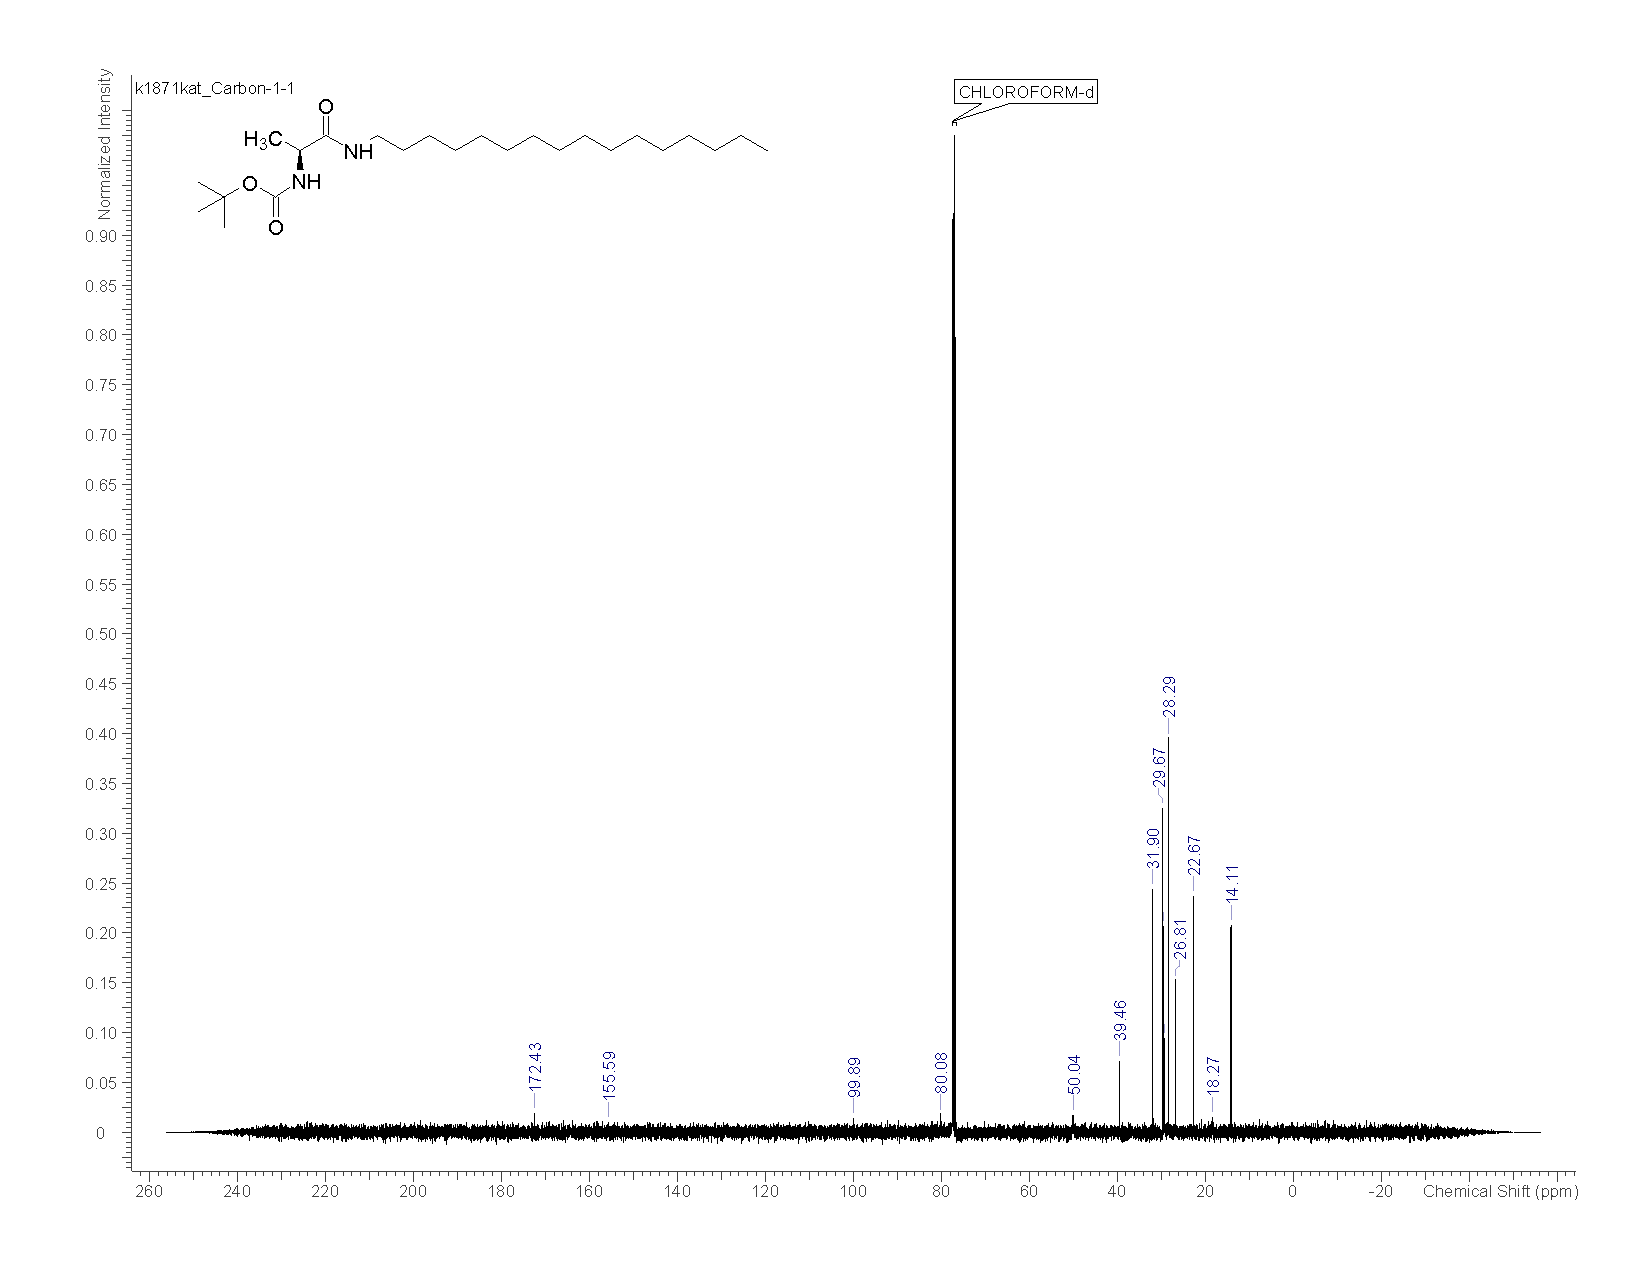
\includegraphics[scale=0.47]{13CNMR/KAT1_23_13C.pdf}
\caption{\textsuperscript{13}C NMR C16-L-Ala(Boc)}
\label{KAT1.23_13C}
\end{figure}